\textit{Physiradio} è un dispositivo IoT (\textit{Internet of Things}) dimostrativo: recupera dalla rete i dati relativi alle condizioni meteo di un luogo scelto in fase di configurazione, li elabora e li rappresenta attraverso una combinazione di musica (genere musicale) e colore. Realizza cioè una possibile ``tangibilizzazione'' (liberamente tradotto dall'inglese \textit{physicalization}) di un dato.
%In particolare, a seconda del tempo atmosferico rilevato, verranno emessi uno specifico genere musicale e uno specifico colore dei led (sotto il prototipo).

\setlength\intextsep{0pt}
\begin{wrapfigure}{r}{0.3\textwidth}
	\vspace{-20pt} % non va tolto!
	\begin{center}
		\includegraphics[width=0.25\textwidth]{Immagini/SCHEMA_PHYSIRADIO.png}
%	\caption{Schema del dispositivo}
	\end{center}
\end{wrapfigure}


Lo scopo di questa demo è raccogliere impressioni su:
\begin{compactitem}
	\item l'idea di rappresentazione del dato atmosferico mediante musica e colori
	\item l'efficacia dello strumento nel sollevare curiosità sulla tecnica di estrazione del dato stesso
\end{compactitem}
\textbf{Nota bene}: non cerchiamo l'associazione perfetta, ci interessa valutare il procedimento di rappresentazione.
%
%%	\begin{figure}[hbt!]
%\begin{center}
%	\includegraphics[width=.4\textwidth]{SCHEMA_PHYSIRADIO.png}
%\end{center}
%%	\end{figure}

Ti chiediamo di compilare il questionario (anonimo) che segue, man mano che procediamo con la dimostrazione,
per fornirci un \textit{feedback} sul lavoro che stiamo realizzando.

%Grazie mille.

\medskip
\hrule
\medskip

%\todo{atrent: preparare proprio il modulo come se fosse cartaceo (anche se poi magari lo compiliamo al pc)}
\begin{compactenum}
	\item Anagrafica (anonima):
	\begin{itemize}
		\item Età [\dots\dots] - Sesso F[~~]~~M[~~] - Città di residenza [\dotfill]
		\item Occupazione [\dotfill]
		\item Titolo di studio: Obbligo[~~]~~Superiori[~~]~~Laurea[~~]~~PhD[~~]
		\item Ascoltatore abituale di musica: Sì[~~]~~No[~~]
		\item Se ``Sì'':
		\begin{compactenum}

			\item Su quale \textit{device}?\newline
			Radio[~~]
			Webradio[~~]
			CD[~~]
			Vinile[~~]
			MP3~player~(o~smartphone~offline)[~~]
			App~streaming[~~]\medskip

			\item In che contesto?\newline
			Casa[~~]
			Lavoro[~~]
			Auto[~~]
			Mezzi~pubblici[~~]
			\newline
			Bagno[~~]
			Letto[~~]
%			\newline
			Allenamento[~~]
			Passeggiando[~~]\newline
			Altro[\dotfill]\medskip

			\item Quali generi musicali ascolti?\newline
			[\dotfill]\newline
			[\dotfill]
		\end{compactenum} 
	
	\end{itemize}

%	\newpage
	
	\item Ora ti faremo ``ascoltare e vedere'' alcune condizioni meteo senza dirti a cosa corrispondono, ti chiediamo per ogni ascolto di inserire uno a o piú X in corrispondenza delle condizioni meteo che meglio lo rappresentano. 
%	Inserisci, per ogni stazione ascoltata (e colore visto), il tempo atmosferico che, secondo te, si è voluto interpretare.
	
\begin{center}
	\begin{tabular}{|c||c|c|c|c|c|c|c|c|c|c|c|c|c|c|c||c|} 
		\hline
		\textbf{Ascolto} &  \rotatebox{90}{\textbf{Pioggia}} & \rotatebox{90}{\textbf{Pioggerella}} & \rotatebox{90}{\textbf{Sereno/Soleggiato}} &  \rotatebox{90}{\textbf{Nuvoloso}} & \rotatebox{90}{\textbf{Temporale}} & \rotatebox{90}{\textbf{Uragano/Nubifragio}} & \rotatebox{90}{\textbf{Tornado}} & \rotatebox{90}{\textbf{Neve}} & 
		\rotatebox{90}{\textbf{Fumo}} & \rotatebox{90}{\textbf{Nebbia}} & \rotatebox{90}{\textbf{Foschia}} & \rotatebox{90}{\textbf{Caligine}} & \rotatebox{90}{\textbf{Sabbia}} & \rotatebox{90}{\textbf{Cenere}} & \rotatebox{90}{\textbf{Polvere}} & \rotatebox{90}{\textbf{Umiditá (Rel.)$\geq$85\% }} \\
		\hline
		\hline
		Ascolto 1 & & & & & & & & & & & & & & & & \\
		\hline
		Ascolto 2 & & & & & & & & & & & & & & & &  \\
		\hline
		Ascolto 3 & & & & & & & & & & & & & & & & \\
		\hline
		Ascolto 4 & & & & & & & & & & & & & & & & \\
		\hline
		Ascolto 5 & & & & & & & & & & & & & & & & \\
		\hline
		Ascolto 6 & & & & & & & & & & & & & & & & \\
		\hline
		Ascolto 7 & & & & & & & & & & & & & & & & \\
%			\hline
%			Ascolto 8 & & & & & & & &  \\
%			\hline
%			Ascolto 9 & & & & & & & &  \\
%			\hline
%			Ascolto 10 & & & & & & & &  \\
		\hline 
		
	\end{tabular}
\end{center} %\todo{atrent: sono 7 ascolti e 8 condizioni meteo...}
	

\item Quale genere musicale e/o colore assoceresti alle seguenti condizioni meteo? (puoi anche compilarla parzialmente: inserisci almeno le associazioni che ti sembrano più calzanti; per aiutarti, puoi anche partire da un genere musicale e associare una condizione meteo)
	\begin{compactitem}
		\item Nebbia [\dotfill]

		\item Pioggia [\dotfill]

		\item Pioggerella [\dotfill]

		\item Sereno/Soleggiato [\dotfill]

		\item Nuvoloso [\dotfill]

		\item Temporale [\dotfill]

		\item Uragano/Nubifragio [\dotfill]

%		\item Inquinato/Polveroso [\dotfill]

		\item Neve [\dotfill]
		
%		++Thunderstorm
%		++Drizzle
%		++Rain
%		++Snow
%		Mist
%		Smoke
%		Haze
%		Dust
%		++Fog
%		Sand
%		Ash
%		++Squall
%		Tornado
%		++Clear
%		++Clouds
		
		%\todo{andare avanti}
	\end{compactitem}
%\todo{[simone]eviterei interamente questa domanda perché possiamo estrapolare questi dati direttamente dalla tabella precedente, la commento solo temporaneamente per vedere il risultato
%- atrent: ribadisco necessità di chiedere una mappatura esplicita, anche perché non credo faremo sentire TUTTE le possibili condizioni, si può chiedere anche una compilazione parziale cioè elencare tutte le condizioni possibili e chiedere di riempire solo quelle di cui ci si sente in grado di consigliare una associazione, parliamone (p.s. il todo va a valle della cosa che devi commentare)
%- atrent: riflettendoci meglio sono convinto che vada messa la domanda, lasciami far valere l'esperienza (ho lavorato alcuni anni in una società che faceva ricerche di mercato)}



%	\item Dimmi il nome di una città! E scrivi il tempo che secondo te c'è adesso in quel posto (non ti abbiamo fatto ascoltare tutte le combinazioni tempo atmosferico-musica possibili).
%	\newline............................................................................................................
	
	
	\item Ritieni efficace/utile la rappresentazione di questo tipo di dato tramite genere musicale e colore?

	%\hrulefill 
	~Poco[~~]~~Abbastanza[~~]~~Molto[~~]~~Moltissimo[~~]

%	\item Riterresti efficace/utile la rappresentazione di un altro tipo di dato (suggerire quale) tramite questo sistema?
%\hrulefill 
%~poco[~~]~~abbastanza[~~]~~molto[~~]~~moltissimo[~~]
%	\item "Ha senso questo tipo di mapping secondo te?” (si/no) .....

	\item Ci suggeriresti un altro tipo di dato interessante da tangibilizzare con questo strumento?\newline
	[\dotfill]\newline
	[\dotfill]
%	\item "Hai in mente qualche altro mapping o esempio d'uso che potrebbero essere sviluppati in futuro?"
%	\newline............................................................................................................


\item \textbf{Open Data}\newline
I dati meteo usati in questo prototipo sono recuperati in tempo reale via rete da fonti cosiddette ``open data'', cioè fonti che forniscono informazioni liberamente utilizzabili tramite programmi (quindi non solo attraverso pagine web). Dentro Physiradio gira infatti un programma che recupera dati dalla rete e sceglie uno \textit{stream} musicale e un colore in base al \textit{mapping} che hai appena sperimentato.

Lo scopo primario del processo di tangibilizzazione è quello di rendere fruibile i dati attraverso vari sensi, ma nel caso particolare di Physiradio ci interessa anche stimolare la curiosità sugli aspetti tecnologici
%e politici 
del mondo dei dati aperti e della trasparenza, cioé:
\begin{compactitem}
	\item Come vengono resi disponibili i dati e come si possono recuperare?
	\item Che forma hanno questi dati e che tipo di elaborazioni/visualizzazioni sono possibili?
%	\item Quali implicazioni socio-politiche ha il tema dell'\textit{opendata}?
\end{compactitem}
Ti abbiamo incuriosito?
~~Poco[~~]~~Abbastanza[~~]~~Molto[~~]~~Moltissimo[~~]
%atrent: questa era relativa all'opendata
%ho tolto i politici che magari qualcuno storce il naso -> [simone] concordo

%ad un utente medio, la possibilità di fruire di un dato "open", ovvero che è reso disponibile e aperto ad analisi e cambiamenti, tramite un mezzo non convenzionale. \newline

%Quindi, è bene sottolineare che questo prototipo non punta a trovare "il mapping perfetto" per i dati messi a disposizione, bensì di mettere le basi (informatiche) per un oggetto, o una categoria di oggetti, IoT che puntano a sfruttare la data physicalization tramite l'udito, attraverso la musica, e la vista.
\end{compactenum}

\hrulefill

\textbf{Commenti liberi:}

[\dotfill]

[\dotfill]

[\dotfill]

[\dotfill]

[\dotfill]

[\dotfill]

[\dotfill]

[\dotfill]

[\dotfill]

\hrulefill

\textbf{GRAZIE!}